\chapter{Hydrostatics}
This chapter is based on Munson Chapter 2.

\section{Pressure at a point}
\label{sec:pressure_at_point}
We commonly assume that pressure at a point is a scalar. However, pressure is the component of stress which is normal to a surface.

We consider a wedge-shaped element of fluid. We apply Newton's force balance to the element, for this we need to transform the pressures acting on the surfaces into forces $F_y,F_z,F_s$. Furthermore, we make the assumption that there are no tangential forces on any of the surfaces: we are neglecting all shearing forces.


\begin{figure}[H]
	\centering
	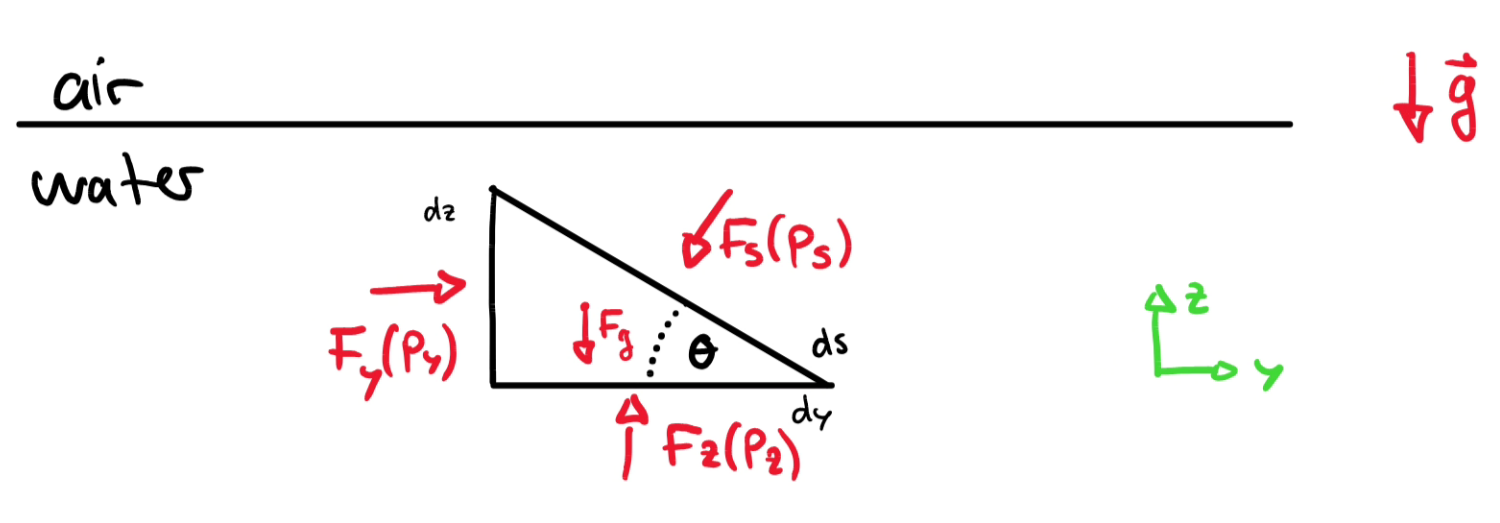
\includegraphics[width=0.6\textwidth]{WedgeElement.png}
	%\caption{}            
\end{figure}

Newton's second law in $z$ direction yields:
\begin{equation*}
	\begin{split}
		\sum \vec F &= m \vec a \\
		\quad F_z = p_z\cdot dx\cdot dy - p_s \cdot ds\cdot dx\cdot \cos \theta-\rho g dV &= \rho dV a_z\qquad \left | \begin{cases}ds = \frac {dy} {\cos\theta}\\ dV = \frac{dz\cdot dy}{2}dx\end{cases}\right.\\
		p_z-p_s -\rho g \frac{dz}2 &= \rho \frac {dz}2a_z\\
		dx,dy,dz\to 0 \implies p_z&=p_s
	\end{split}
\end{equation*}
Similarly we can do the calculation in $x$ and $y$, which results in a final result of
$$
p_z=p_x=p_y=p_s
$$
for any angle $\theta$.

Seeing that the pressure is equal for any direction, we can conclude that $p$ is a scalar
\section{Equation for Pressure Field}
Using the same idea as for \ref{sec:pressure_at_point}, we look at a box.
\begin{figure}[H]
	\centering
	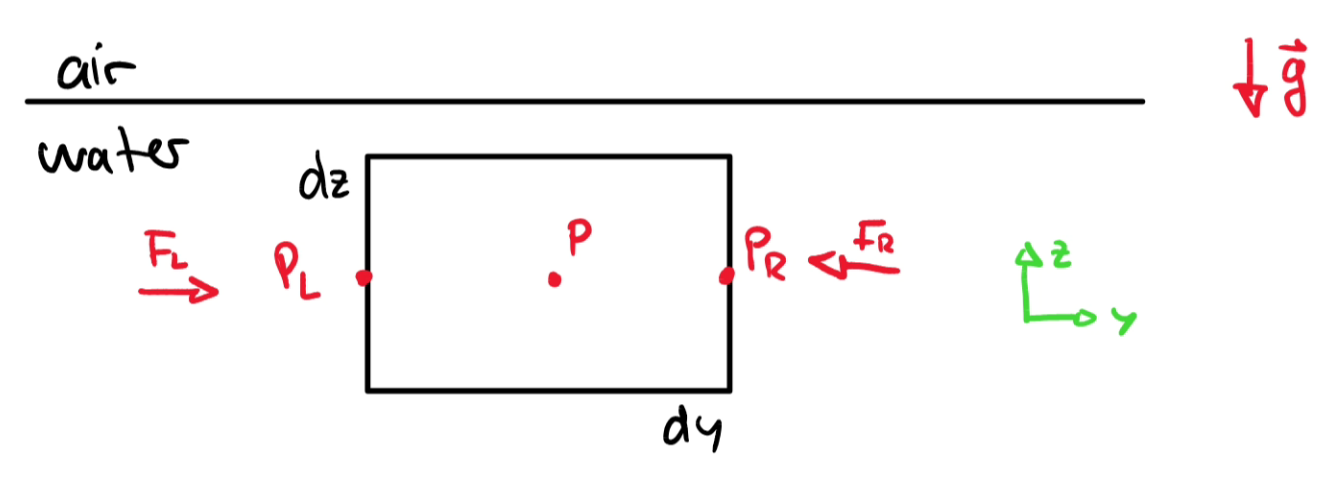
\includegraphics[width=0.6\textwidth]{CubeElement.png}
	%\caption{}            
\end{figure}
We use Taylor expansion to express $p_l$ and $p_r$:
\begin{equation*}
	\begin{split}
		p_r &= p + \left.\frac{dy}{2}\frac{\partial p}{\partial y}\right|_0+\dots\\
		p_l &= p - \left.\frac{dy}{2}\frac{\partial p}{\partial y}\right|_0+\dots\\
		\implies F_R &= p_r\cdot dx\cdot dz = \left( p + \left. \frac{dy}{2}\frac{\partial p}{\partial y}\right|_0\right)dx\cdot dy+\dots\\
		\implies F_L &= p_l\cdot dx\cdot dz = \left( p - \left. \frac{dy}{2}\frac{\partial p}{\partial y}\right|_0\right)dx\cdot dy+\dots\\
	\end{split}
\end{equation*}
We apply force balance in $y$:
\begin{equation*}
	\begin{split}
		-F_R+F_L&=\rho dVa_y\\
		\left.-dy\frac{\partial p}{\partial y}\right|_0\cdot dx\cdot dz &= \rho\cdot dx\cdot dy\cdot dz\cdot a_y+\dots \\
		-\left.\frac{\partial p}{\partial y}\right|_0&=\rho a_y+\dots
		\stackrel{\lim_{dx,dy,dz\to 0 }}{\implies}\left.-\frac{\partial p}{\partial y}\right|_0=\rho a_y
	\end{split}
\end{equation*}
We could do the same calculation in the $x$ and $z$ direction, where the weight needs to be considered. We can rewrite Newtons second law per unit volume:
\begin{equation}
	\boxed{-\nabla p -\rho g\hat k =\rho \vec a}
	\label{eq:newtons_second_law_per_unit_volume}
\end{equation}
\paragraph{Remark} Remember that we neglected shear forces to derive this result. It is only valid if we have no shear forces.

\section{Fluids at Rest}
When a fluid is at rest, from newtons second law we can say that $\vec a = \vec 0$. The derived equation for newton seconds law per unit volume \eqref{eq:newtons_second_law_per_unit_volume} then yields:
\begin{equation}
	\begin{split}
		-\frac{\partial p}{\partial x} &= 0\\
		-\frac{\partial p}{\partial y} &= 0\\
		-\frac{\partial p}{\partial z}-\rho g &= 0
	\end{split}
	\label{eq:fluid_at_rest}
\end{equation}
Which means that the pressure only depends on $z$:
$$
p = p(z)
$$
We can solve the differential equation in \eqref{eq:fluid_at_rest} to find the pressure function explicitly:
\begin{equation}
	\begin{split}
		\frac{\partial p}{\partial z} &= -\rho g\\
		\int dp &= - \int \rho g dz\\
		\Delta p &\stackrel{(*)}{=} - g \int \rho\, dz
	\end{split}
	\label{eq:pressure_difference}
\end{equation}
Where at $(*)$ we assumed the gravitational acceleration to be constant.
\subsubsection{Incompressible Fluid}
If $\rho$ is constant, a fluid is considered to be an incompressible fluid. The equation for pressure difference \eqref{eq:pressure_difference} is simple to solve:
\begin{equation*}
	\Delta p = -g\rho \Delta z
\end{equation*}
Choosing a coordinate system that goes down with $h$ (height below reference surface) and has its origin such that $h_0=0$ at $p_0$ we can reorder
\begin{equation}
	\boxed{p(h)=\rho g h + p_h}
	\label{eq:pressure_incompressible}
\end{equation}
\paragraph{Remark}

Remember that $p$ is absolute pressure, relative to vacuum. Compared to gage pressure, which is relative to a reference pressure such as the atmospheric pressure. Gage pressure in the above equation \eqref{eq:pressure_incompressible} would be $p-p_h = \rho g h$
